\documentclass[12pt,a4paper]{article}

% ---------------------------------------------------------
% Packages & Environment Setup
% ---------------------------------------------------------
\usepackage[utf8]{inputenc}
\usepackage[margin=1in]{geometry}
\usepackage{amsmath,amssymb,amsfonts}
\usepackage{graphicx}
\usepackage{xcolor}
\usepackage{hyperref}
\usepackage{booktabs}
\usepackage{multirow}
\usepackage{listings}
\usepackage{caption}
\usepackage{subcaption}
\usepackage{fancyhdr}
\usepackage{tcolorbox}
\usepackage{tikz}
\usetikzlibrary{shapes.geometric, arrows.meta, positioning, shadows}

% ---------------------------------------------------------
% Formatting & Color Definitions
% ---------------------------------------------------------
\definecolor{primaryblue}{RGB}{21, 101, 192}
\definecolor{darknavy}{RGB}{27, 42, 61}
\definecolor{accentcyan}{RGB}{0, 172, 193}
\definecolor{codebg}{RGB}{245, 247, 250}
\definecolor{codecomment}{RGB}{100, 116, 139}

\hypersetup{
    colorlinks=true,
    linkcolor=primaryblue,
    filecolor=primaryblue,      
    urlcolor=primaryblue,
    citecolor=primaryblue
}

\lstset{
    backgroundcolor=\color{codebg},
    basicstyle=\ttfamily\footnotesize,
    breaklines=true,
    captionpos=b,
    commentstyle=\color{codecomment},
    keywordstyle=\color{primaryblue}\bfseries,
    stringstyle=\color{accentcyan},
    frame=single,
    rulecolor=\color{lightgray}
}

% tcolorbox setup for User Guide Note Boxes
\tcbuselibrary{skins,breakable}
\newtcolorbox{guidebox}[2][]{
    colback=white,
    colframe=primaryblue,
    fonttitle=\bfseries\color{white},
    title=#2,
    enhanced,
    attach boxed title to top left={xshift=3mm,yshift=-3mm},
    boxed title style={colback=primaryblue},
    #1
}

% Header and Footer Setup
\pagestyle{fancy}
\fancyhf{}
\rhead{\color{codecomment}\small NetFix Platform User Guide}
\lhead{\color{primaryblue}\bfseries NetFix Anomaly \& 5G Planning}
\rfoot{\thepage}

% ---------------------------------------------------------
% DOCUMENT START
% ---------------------------------------------------------
\begin{document}

\title{\textbf{\Huge NetFix Unified Platform}\\
\Large Technical User Manual \& Comprehensive Operational Guide\\
\large Grounded UI Workflow Documentation for Optimization \& Planning Engineers}
\author{\textbf{NetFix Core Engineering Team}}
\date{\today}

\maketitle
\tableofcontents
\newpage

% =========================================================
\section{Platform Introduction \& Role-Based Architecture}
% =========================================================
The \textbf{NetFix Unified Telecommunication Platform} integrates two distinct, enterprise-grade mobile network engineering portals into a single single-pane-of-glass web application:
\begin{enumerate}
    \item \textbf{NetFix Anomaly Detection Portal:} A multi-model statistical, Histogram Gradient Boosting ML, and PyTorch LSTM temporal fusion platform combined with a 34-reason deterministic Root Cause Analysis (RCA) engine, interactive Leaflet GIS trajectory mapping, and a local quantized LLM AI Assistant (\textbf{Penguin AI}).
    \item \textbf{NetFix 5G Planning Portal (NetPulse):} A spatial geometry, neighbor graph, and constraint satisfaction engine for allocating 5G NR Physical Cell Identifiers (PCI), Root Sequence Indices (RSI), and PRACH parameters while enforcing strict modulo (Mod3, Mod4, Mod30) conflict rules.
\end{enumerate}

The platform implements a strict \textbf{Role-Based Access Control (RBAC)} and dynamic forwarding model upon user login:
\begin{itemize}
    \item \textbf{Optimization Engineer Role:} Automatically forwards to the \textbf{NetFix Anomaly Detection Portal} (\texttt{/dashboard}).
    \item \textbf{Planning Engineer Role:} Automatically forwards to the \textbf{NetFix 5G Planning Portal} (\texttt{/np-upload}).
\end{itemize}

\newpage

% =========================================================
\section{NetFix Anomaly Detection \& Troubleshooting Portal}
% =========================================================

\begin{guidebox}{Target Persona: Optimization Engineer / RF Performance Specialist}
This chapter provides an exhaustive, step-by-step operational manual for Radio Access Network (RAN) Optimization Engineers. Grounded strictly in actual UI screenshots of the \textbf{NetFix Anomaly Detection Portal}, this document details every navigation module, KPI widget, pipeline progress stepper, deterministic root-cause breakdown, GIS map interface, and interactive AI Copilot workflow.
\end{guidebox}

\subsection{System Navigation and Portal Layout Framework}
The NetFix interface is structured around a persistent dark-navy primary navigation sidebar (\texttt{\#1B2A3D}) and an enterprise light workspace area (\texttt{\#F8FAFC}):
\begin{enumerate}
    \item \textbf{NETFIX ANALYSIS Module Group:}
    \begin{itemize}
        \item \textbf{Dashboard:} Real-time overall telemetry health overview, KPI metric cards, severity distributions, and high-resolution ML backend time-series figures.
        \item \textbf{Upload Dataset:} Ingestion dropzone for raw \texttt{.pkl} network drive-test payloads with 4-stage execution stepper and recent session audit log.
        \item \textbf{Results:} Root Cause Analysis (RCA) engine, 23-metric telemetry breakdown grids, 3GPP standard references, and vendor resolution steps.
        \item \textbf{Interactive Map:} High-performance Leaflet GIS canvas plotting drive-test GPS breadcrumbs, cell towers, and pinpoint anomaly markers.
    \end{itemize}
    \item \textbf{INSIGHTS Module Group:}
    \begin{itemize}
        \item \textbf{Reports:} Automated PDF diagnostic summaries and exported data profiling figures.
        \item \textbf{Penguin AI:} Conversational AI Engineering Copilot powered by local quantized LLMs (\texttt{llama3.1}, \texttt{deepseek-r1}) for deep technical reasoning and grounded report generation.
    \end{itemize}
    \item \textbf{SYSTEM Module Group:}
    \begin{itemize}
        \item \textbf{History:} Audit log tracking all historical analysis sessions, completion statuses, anomaly counts, and cause-matching totals.
        \item \textbf{Settings:} Threshold configuration defaults, model selection preferences, and API endpoints.
    \end{itemize}
    \item \textbf{User Context Badge (Bottom-Left):} Displays logged-in engineer credentials (\texttt{Mego 312002}, \texttt{Optimization Eng.}), active role badge, and session logout controls.
\end{enumerate}

---

\subsection{Module 1: Telemetry Overview \& ML Pipeline Dashboard}
\textit{Reference Screenshot: \texttt{Screenshot from 2026-08-12 14-38-38.png}}

The \textbf{Dashboard} view serves as the primary operational landing page after portal authentication. It consolidates dataset-wide telemetry metrics and machine learning validation plots:

\begin{figure}[htbp]
\centering
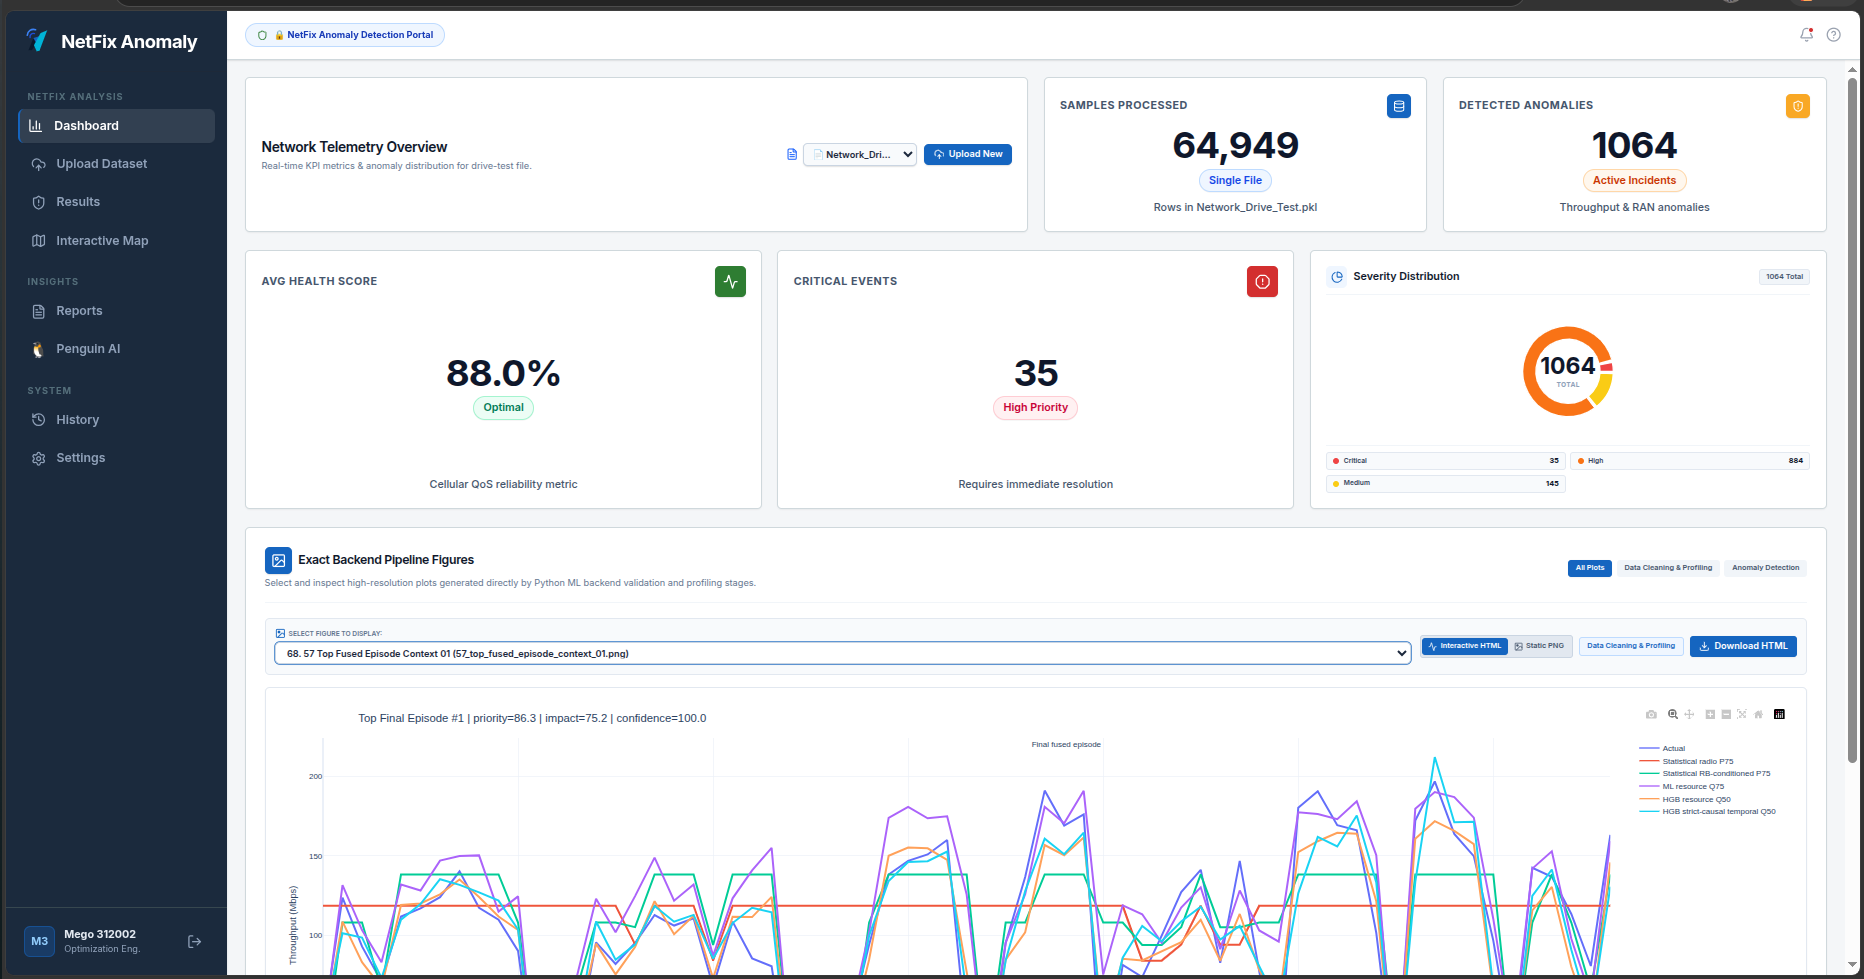
\includegraphics[width=0.95\textwidth]{images/Screenshot from 2026-08-12 14-38-38.png}
\caption{NetFix Anomaly Dashboard displaying live telemetry metrics, 1,064 detected incidents, severity donut distribution, and interactive backend pipeline time-series figures.}
\label{fig:ug_dashboard}
\end{figure}

\subsubsection{Top Telemetry Metric Cards}
\begin{table}[htbp]
\centering
\caption{Dashboard Telemetry Overview Metric Specifications.}
\label{tab:dash_metrics_ug}
\small
\begin{tabular}{llp{7.5cm}}
\toprule
\textbf{Metric Card Title} & \textbf{Observed Value} & \textbf{Technical Description \& Scope} \\
\midrule
\textbf{SAMPLES PROCESSED} & \textbf{64,949} & Total telemetry measurement rows loaded from \texttt{Network\_Drive\_Test.pkl}. Marked with \texttt{Single File} badge. \\
\textbf{DETECTED ANOMALIES} & \textbf{1,064} & Total active incident episodes detected across throughput and radio parameters. Marked with \texttt{Active Incidents} badge. \\
\textbf{AVG HEALTH SCORE} & \textbf{88.0\%} & Cellular Quality of Service (QoS) reliability score. Marked with green \texttt{Optimal} health status badge. \\
\textbf{CRITICAL EVENTS} & \textbf{35} & High-priority operational anomalies requiring immediate engineering resolution. Marked with red alert icon. \\
\bottomrule
\end{tabular}
\end{table}

\subsubsection{Severity Distribution Analytics}
The dashboard features an interactive donut chart breaking down the 1,064 detected incidents by operational severity:
\begin{itemize}
    \item \textbf{Critical (Red):} 35 incidents ($3.3\%$). Severe throughput drop or radio link failure.
    \item \textbf{High (Orange):} 884 incidents ($83.1\%$). Significant throughput degradation below statistical P75.
    \item \textbf{Medium (Yellow):} 145 incidents ($13.6\%$). Moderate KPI variance or localized cell-edge drops.
\end{itemize}

\subsubsection{Exact Backend Pipeline Figures Panel}
Allows engineers to inspect high-resolution validation figures generated by the Python ML backend:
\begin{itemize}
    \item \textbf{Figure Selection Dropdown:} Allows selecting generated artifacts (e.g., \texttt{68. 57 Top Fused Episode Context 01 (57\_top\_fused\_episode\_context\_01.png)}).
    \item \textbf{View Mode Triggers:} Toggle between \textbf{Interactive HTML}, \textbf{Static PNG}, \textbf{Data Cleaning \& Profiling}, and \textbf{Download HTML}.
    \item \textbf{Plot Axis \& Legend Breakdown:} Plots Throughput ($0$--$200$ Mbps) against sequence index:
    \begin{itemize}
        \item \texttt{Actual Throughput} (Solid cyan line): Live recorded mobile payload speed.
        \item \texttt{Statistical radio P75} (Red baseline): 75th percentile expected throughput based on cell radio state.
        \item \texttt{Statistical RB-conditioned P75} (Orange baseline): Resource-block conditioned expected throughput.
        \item \texttt{ML resource Q75} (Purple curve): 75th percentile quantile regression from ML feature space.
        \item \texttt{HGB resource Q50} (Yellow curve): Histogram Gradient Boosting median resource expectation.
        \item \texttt{HGB strict-causal temporal Q50} (Blue curve): Strict-causal temporal sequence prediction.
    \end{itemize}
\end{itemize}

---

\subsection{Module 2: Dataset Ingestion \& 4-Stage Stepper}
\textit{Reference Screenshot: \texttt{Screenshot from 2026-08-12 14-38-48.png}}

The \textbf{Upload Dataset} page orchestrates file ingestion and real-time execution feedback.

\begin{figure}[htbp]
\centering
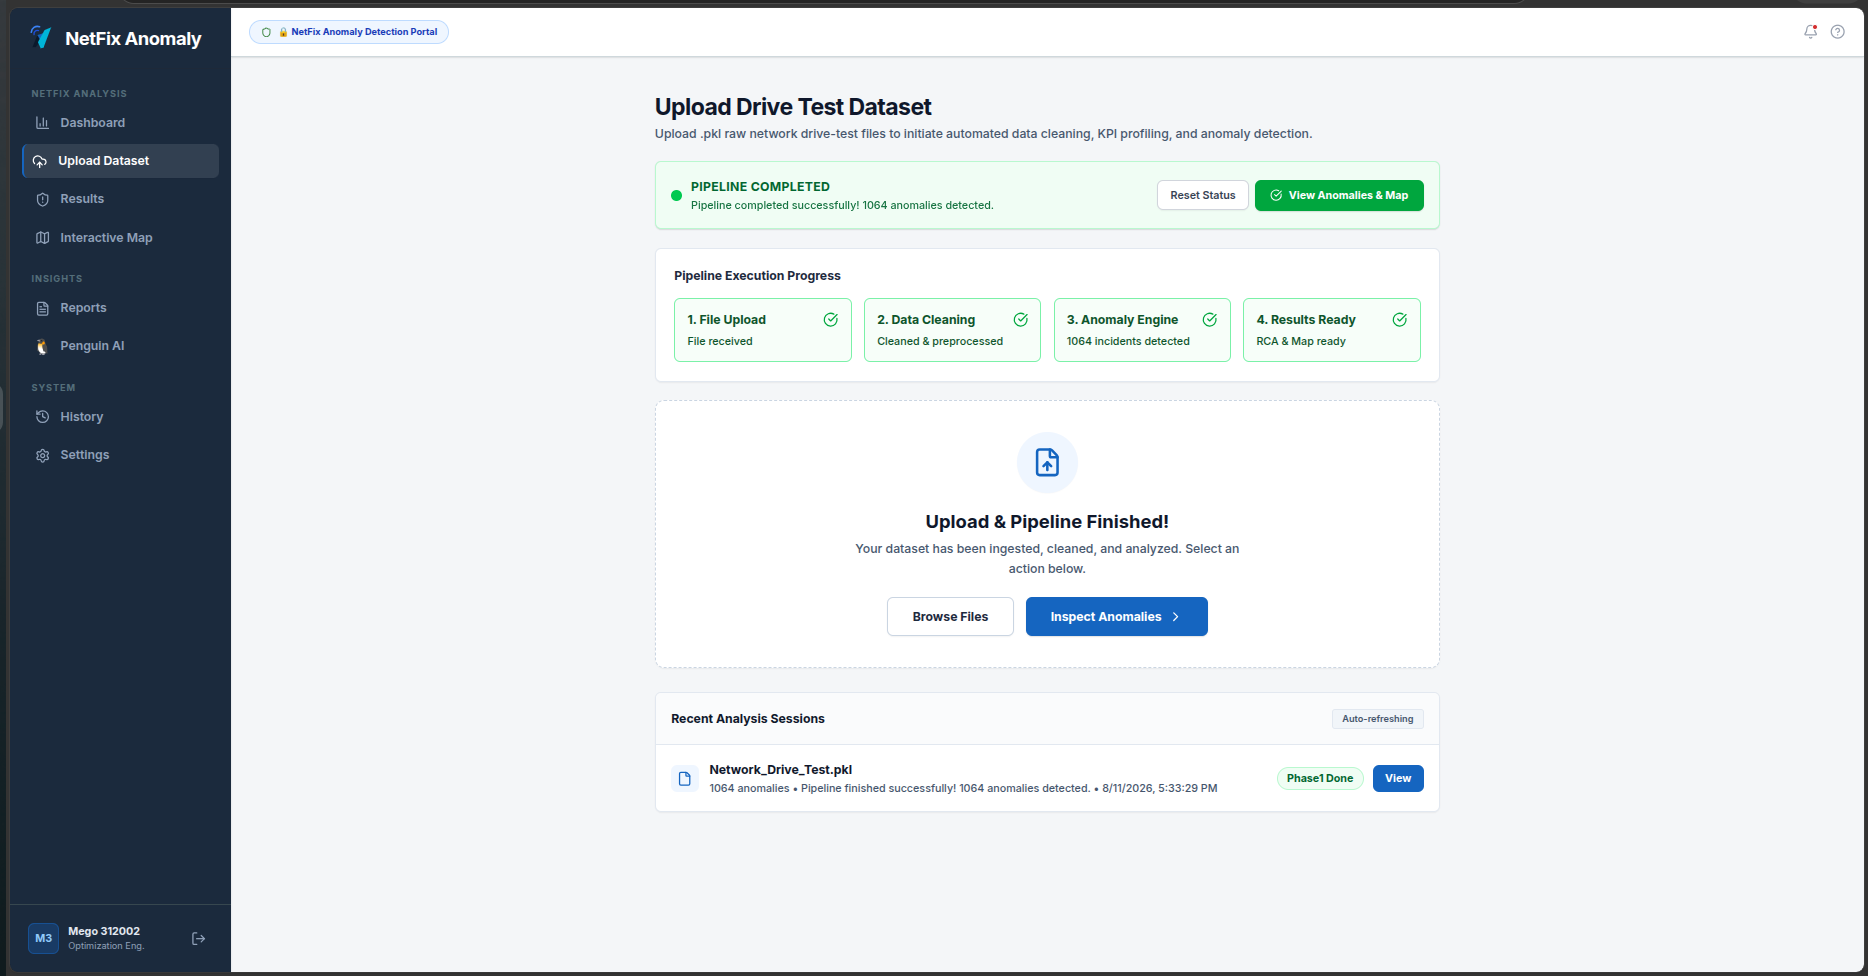
\includegraphics[width=0.95\textwidth]{images/Screenshot from 2026-08-12 14-38-48.png}
\caption{Upload Dataset page showing 4-stage execution stepper (File Upload, Data Cleaning, Anomaly Engine, Results Ready) and recent session audit log.}
\label{fig:ug_upload}
\end{figure}

\subsubsection{4-Stage Execution Progress Stepper}
\begin{enumerate}
    \item \textbf{1. File Upload (Completed $\checkmark$):} Validates file payload integrity and receives raw \texttt{.pkl} network drive-test file.
    \item \textbf{2. Data Cleaning (Completed $\checkmark$):} Executes 11-stage non-leaking preprocessing pipeline (\texttt{ran-cleaning-service}).
    \item \textbf{3. Anomaly Engine (Completed $\checkmark$):} Runs 19-stage statistical, HGB ML, and PyTorch LSTM anomaly fusion models (\textbf{1,064 incidents detected}).
    \item \textbf{4. Results Ready (Completed $\checkmark$):} Constructs MongoDB session indexes and prepares RCA cause-matching and GIS map artifacts.
\end{enumerate}

\subsubsection{Pipeline Completed Banner \& Controls}
Upon completion, a green status banner displays:
\begin{center}
\texttt{PIPELINE COMPLETED ── Pipeline completed successfully! 1064 anomalies detected.}
\end{center}
Engineers can click \textbf{View Anomalies \& Map} to jump directly to the GIS map or \textbf{Reset Status} to prepare for a new file upload.

\subsubsection{Recent Analysis Sessions Audit Log}
Displays active sessions in a clean tabular view containing Dataset Name (\texttt{Network\_Drive\_Test.pkl}), Anomaly Count (\texttt{1064 anomalies}), Timestamp (\texttt{8/11/2026, 5:33:29 PM}), Pipeline Status Badge (\texttt{Phase1 Done}), and a direct \textbf{View} session button.

---

\subsection{Module 3: Deterministic RCA Engine \& Telemetry Evidence}
\textit{Reference Screenshots: \texttt{Screenshot from 2026-08-12 14-39-04.png} \& \texttt{14-39-08.png}}

The \textbf{Results} view provides deep-dive root cause analysis for individual anomaly incidents.

\begin{figure}[htbp]
\centering
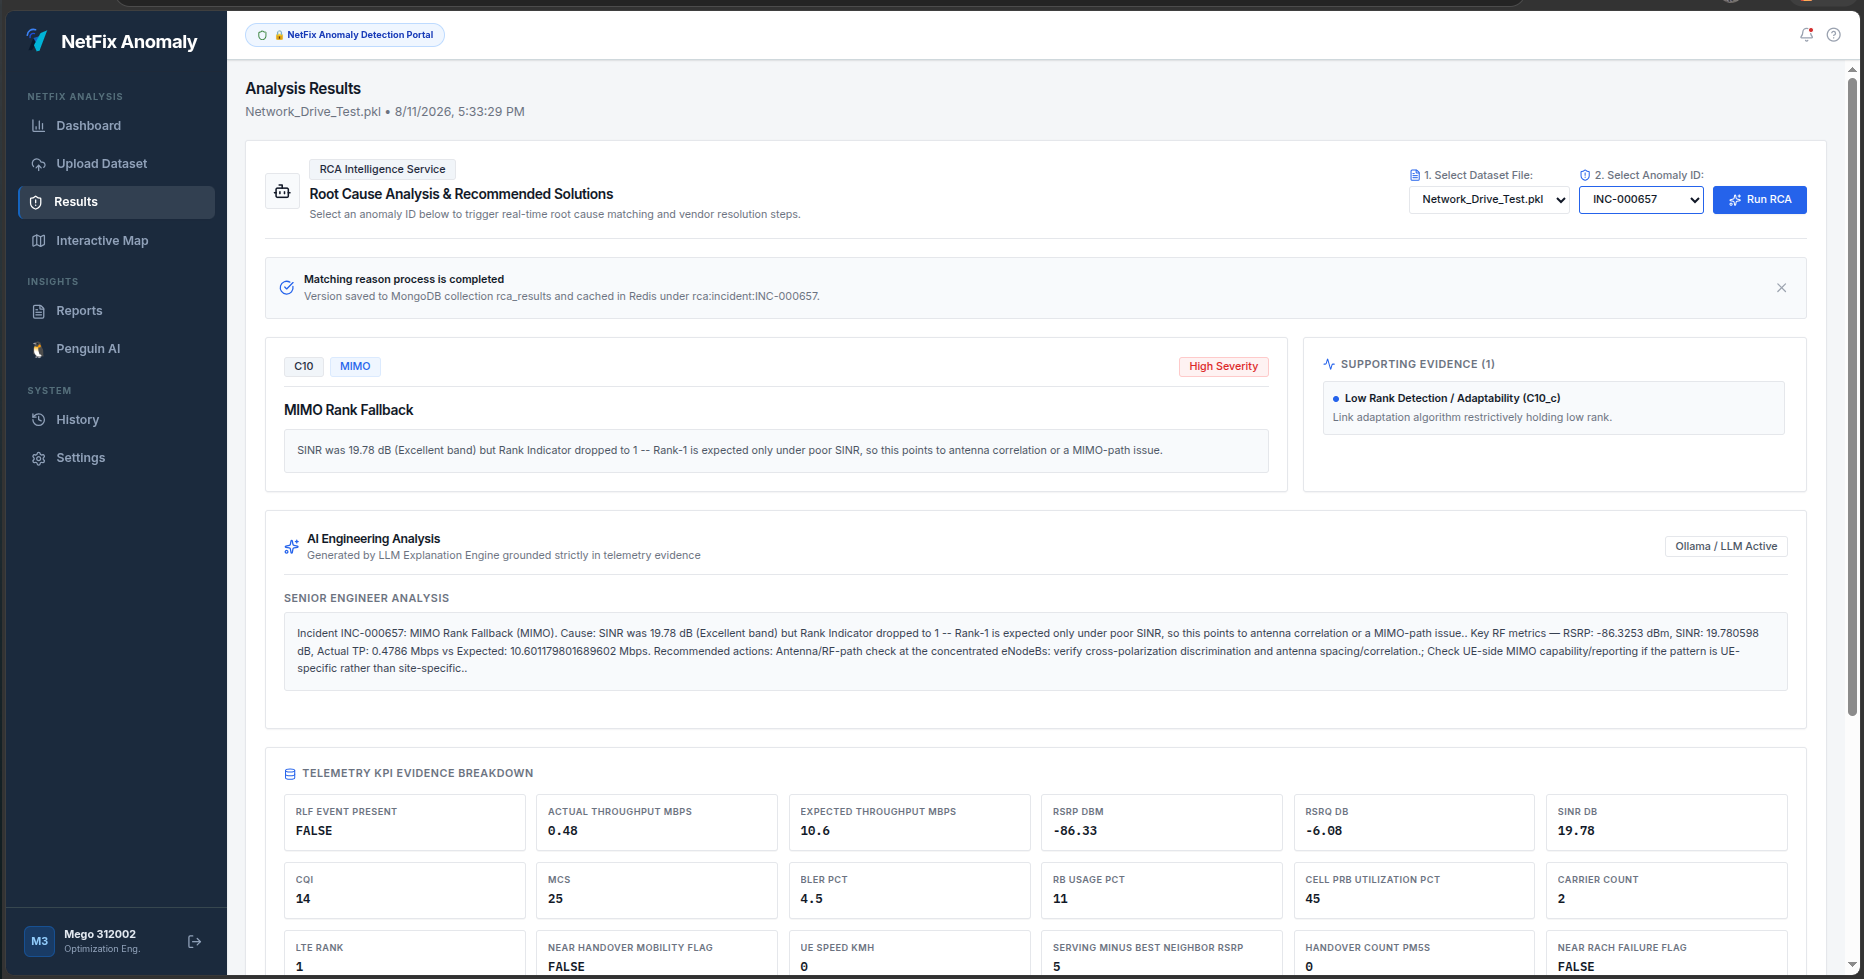
\includegraphics[width=0.95\textwidth]{images/Screenshot from 2026-08-12 14-39-04.png}
\caption{Results page displaying matched rule card (C10 MIMO Rank Fallback), Ollama AI Senior Engineer analysis, and 23-metric telemetry evidence breakdown grid.}
\label{fig:ug_rca_grid}
\end{figure}

\begin{figure}[htbp]
\centering
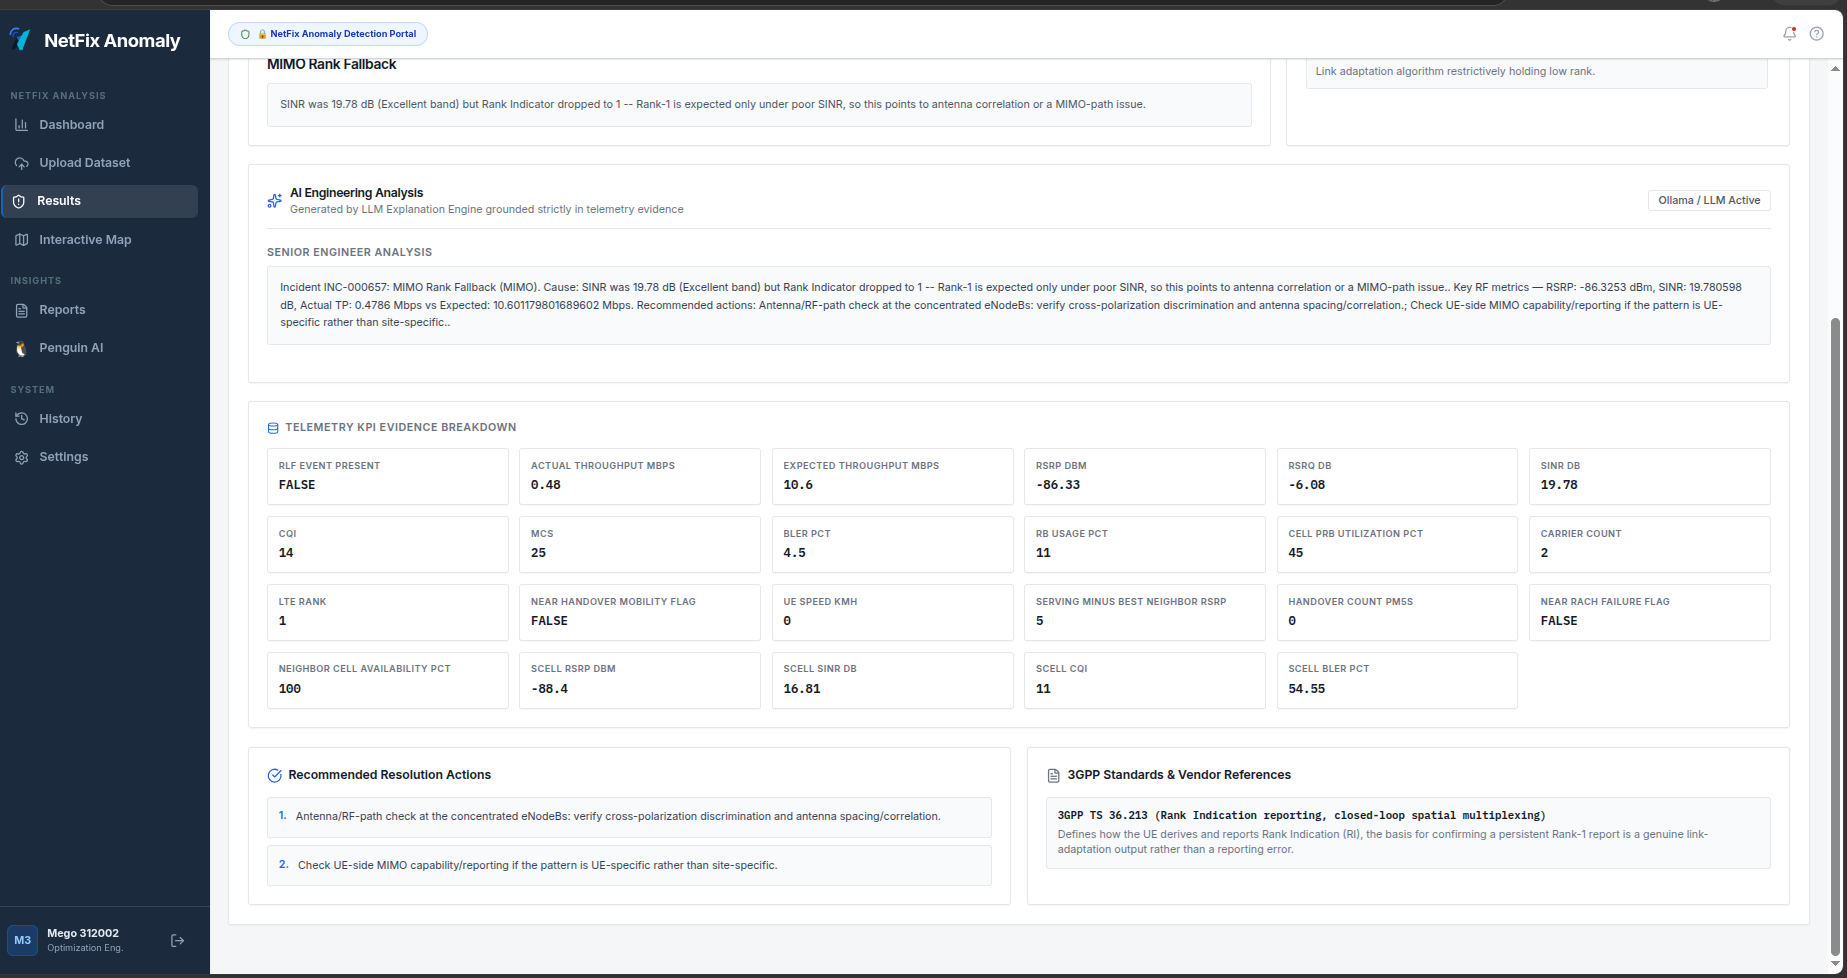
\includegraphics[width=0.95\textwidth]{images/Screenshot from 2026-08-12 14-39-08.png}
\caption{Results page displaying recommended resolution actions and official 3GPP TS 36.213 standards reference.}
\label{fig:ug_rca_recs}
\end{figure}

\subsubsection{Incident Selection Header}
Engineers select the target dataset (\texttt{Network\_Drive\_Test.pkl}) and target Incident ID (e.g., \texttt{INC-000657}) via drop-down selectors, then click \textbf{Run RCA}. A status confirmation banner verifies:
\begin{center}
\small\texttt{Matching reason process is completed ── Version saved to MongoDB collection rca\_results and cached in Redis under rca:incident:INC-000657.}
\end{center}

\subsubsection{Rule-Based Match Card (e.g., Incident INC-000657)}
\begin{itemize}
    \item \textbf{Category \& Badges:} \texttt{C10}, \texttt{MIMO}, \texttt{High Severity}.
    \item \textbf{Matched Reason Title:} \textbf{MIMO Rank Fallback}
    \item \textbf{Cause Narrative:} \textit{``SINR was 19.78 dB (Excellent band) but Rank Indicator dropped to 1 -- Rank-1 is expected only under poor SINR, so this points to antenna correlation or a MIMO-path issue.''}
    \item \textbf{Supporting Evidence Panel:} \texttt{Low Rank Detection / Adaptability (C10\_c)}: Link adaptation algorithm restrictively holding low rank despite clean RF conditions.
\end{itemize}

\subsubsection{AI Engineering Analysis Card (Local Ollama Engine)}
Synthesizes grounded commentary combining ML metrics and physical layer phenomena:
\begin{quote}
\small
\textbf{SENIOR ENGINEER ANALYSIS:} Incident INC-000657: MIMO Rank Fallback (MIMO). Cause: SINR was 19.78 dB (Excellent band) but Rank Indicator dropped to 1 -- Rank-1 is expected only under poor SINR, so this points to antenna correlation or a MIMO-path issue. Key RF metrics — RSRP: -86.3253 dBm, SINR: 19.780598 dB, Actual TP: 0.4786 Mbps vs Expected: 10.601179 Mbps. Recommended actions: Antenna/RF-path check at the concentrated eNodeBs: verify cross-polarization discrimination and antenna spacing/correlation; Check UE-side MIMO capability/reporting if the pattern is UE-specific rather than site-specific.
\end{quote}

\subsubsection{23-Metric Telemetry Evidence Breakdown Grid}
Presents a complete 23-card telemetry metric grid extracted from MongoDB for the exact anomaly timestamp:
\begin{table}[htbp]
\centering
\caption{Incident INC-000657 Telemetry Evidence Grid Breakdown.}
\label{tab:inc_657_grid_ug2}
\small
\begin{tabular}{lll}
\toprule
\textbf{Telemetry Metric Field} & \textbf{Recorded Value} & \textbf{Evaluation \& State} \\
\midrule
\texttt{RLF EVENT PRESENT} & \textbf{FALSE} & No Radio Link Failure event. \\
\texttt{ACTUAL THROUGHPUT MBPS} & \textbf{0.48 Mbps} & Severe degradation (Expected: 10.6 Mbps). \\
\texttt{EXPECTED THROUGHPUT MBPS} & \textbf{10.6 Mbps} & Calculated P75 baseline for cell. \\
\texttt{RSRP DBM} & \textbf{-86.33 dBm} & Good serving cell signal strength. \\
\texttt{RSRQ DB} & \textbf{-6.08 dB} & Good serving cell signal quality. \\
\texttt{SINR DB} & \textbf{19.78 dB} & Excellent Signal-to-Interference Ratio. \\
\texttt{CQI} & \textbf{14} & High Channel Quality Indicator (64QAM/256QAM). \\
\texttt{MCS} & \textbf{25} & High Modulation \& Coding Scheme index. \\
\texttt{BLER PCT} & \textbf{4.5\%} & Low Block Error Rate ($<5\%$). \\
\texttt{RB USAGE PCT} & \textbf{11\%} & Low Resource Block usage. \\
\texttt{CELL PRB UTILIZATION PCT} & \textbf{45\%} & Moderate Cell load. \\
\texttt{CARRIER COUNT} & \textbf{2} & Dual Component Carrier (CA active). \\
\texttt{LTE RANK} & \textbf{1} & \textbf{ANOMALOUS (Rank 1 under 19.78 dB SINR)}. \\
\texttt{NEAR HANDOVER MOBILITY FLAG} & \textbf{FALSE} & Stationary / Low mobility state. \\
\texttt{UE SPEED KMH} & \textbf{0 km/h} & Stationary User Equipment. \\
\texttt{SERVING MINUS BEST NEIGHBOR RSRP} & \textbf{5 dB} & Adequate cell dominance margin. \\
\texttt{HANDOVER COUNT PM5S} & \textbf{0} & No recent handovers. \\
\texttt{NEAR RACH FAILURE FLAG} & \textbf{FALSE} & Random Access Channel normal. \\
\texttt{NEIGHBOR CELL AVAILABILITY PCT} & \textbf{100\%} & All neighbor cells available. \\
\texttt{SCELL RSRP DBM} & \textbf{-88.4 dBm} & Secondary Cell RSRP clean. \\
\texttt{SCELL SINR DB} & \textbf{16.81 dB} & Secondary Cell SINR clean. \\
\texttt{SCELL CQI} & \textbf{11} & Secondary Cell CQI acceptable. \\
\texttt{SCELL BLER PCT} & \textbf{54.55\%} & Secondary Cell BLER elevated. \\
\bottomrule
\end{tabular}
\end{table}

\subsubsection{Recommended Actions \& 3GPP Standard References}
\begin{enumerate}
    \item \textbf{Action 1:} Antenna/RF-path check at concentrated eNodeBs: verify cross-polarization discrimination and antenna spacing/correlation.
    \item \textbf{Action 2:} Check UE-side MIMO capability/reporting if the pattern is UE-specific rather than site-specific.
    \item \textbf{3GPP Standard Reference:} \textbf{3GPP TS 36.213 (Rank Indication reporting, closed-loop spatial multiplexing)}: Defines how the UE derives and reports Rank Indication (RI), the basis for confirming a persistent Rank-1 report is a genuine link-adaptation output rather than a reporting error.
\end{enumerate}

---

\subsection{Module 4: Interactive GIS Trajectory Map}
\textit{Reference Screenshot: \texttt{Screenshot from 2026-08-12 14-39-17.png}}

The \textbf{Interactive Map} view renders geospatial drive-test trajectories over an interactive Leaflet canvas.

\begin{figure}[htbp]
\centering
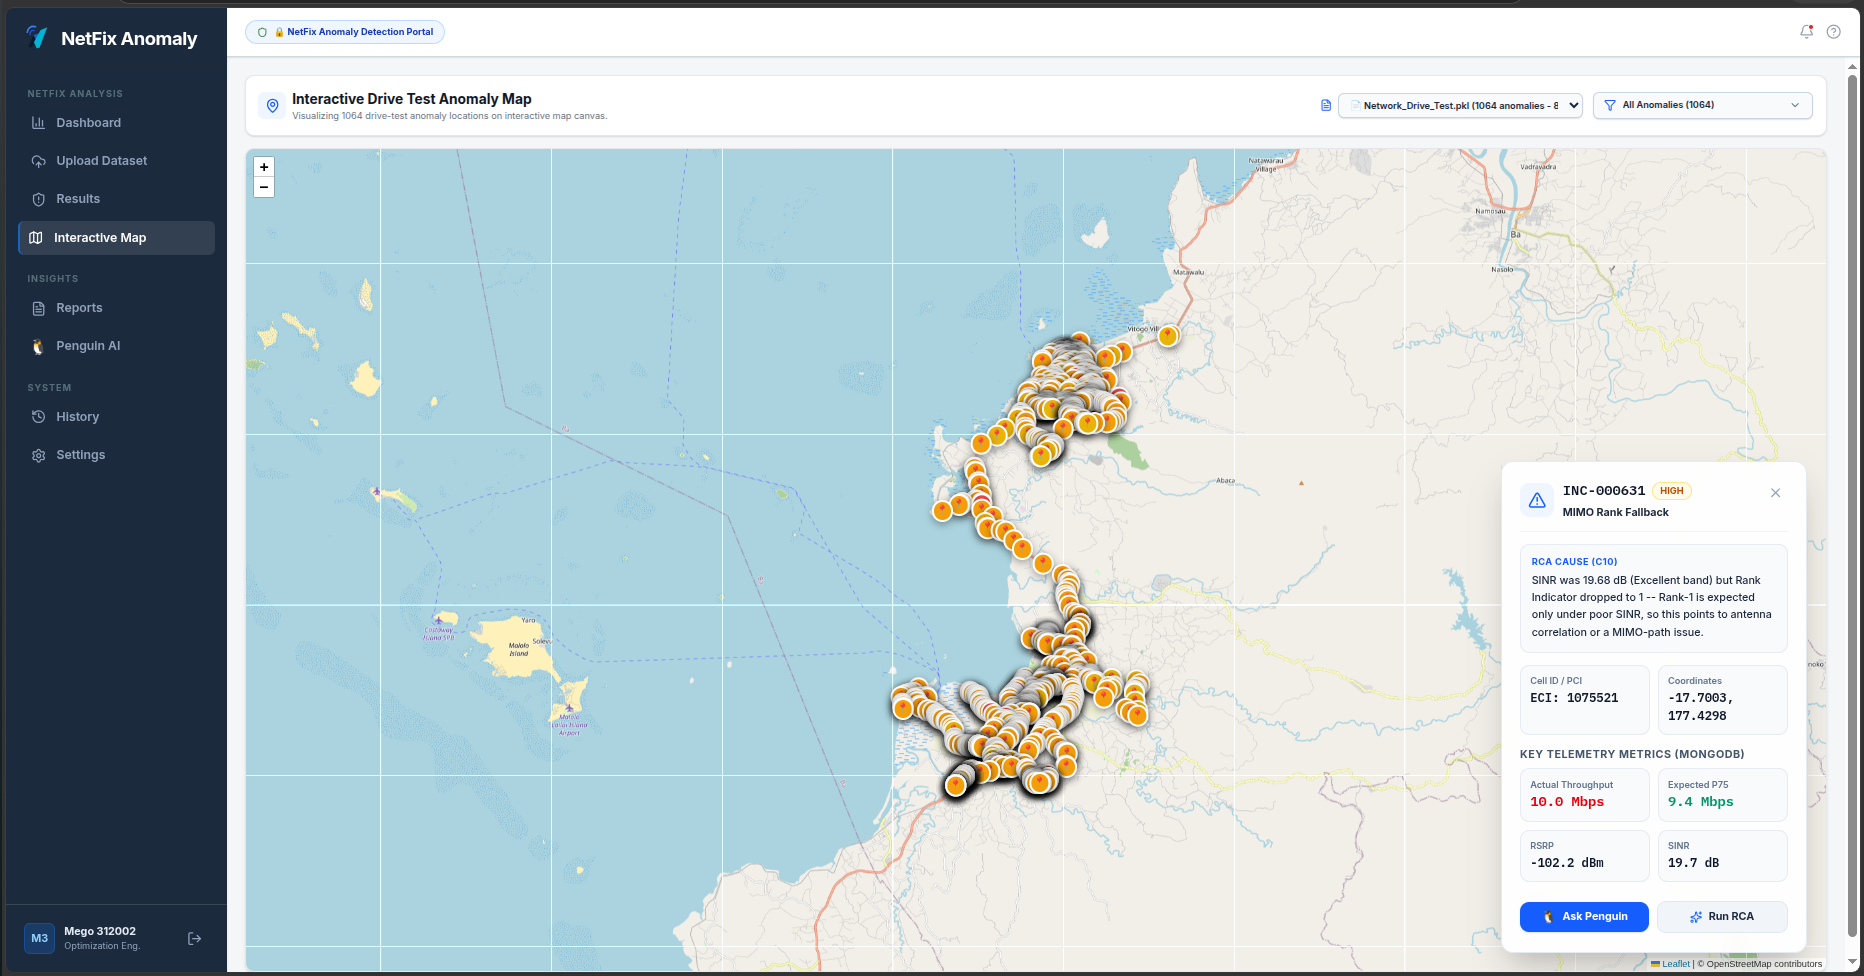
\includegraphics[width=0.95\textwidth]{images/Screenshot from 2026-08-12 14-39-17.png}
\caption{Interactive Map view showing GPS drive-test breadcrumb path, anomaly pin markers, and interactive popup for Incident INC-000631.}
\label{fig:ug_map}
\end{figure}

\subsubsection{Map Controls \& Layer Filters}
\begin{itemize}
    \item \textbf{Dataset Selector:} Switch active dataset file (\texttt{Network\_Drive\_Test.pkl}).
    \item \textbf{Incident Filter Dropdown:} Filter displayed markers (\texttt{All Anomalies (1064)} or specific severity tiers).
    \item \textbf{Zoom \& Canvas Navigation:} Full pan/zoom capabilities with custom OpenStreetMap tile rendering.
\end{itemize}

\subsubsection{Drive-Test Trajectory \& Pinplot Inspection}
The drive path is rendered as a continuous GPS breadcrumb line along coastal highway routes. Anomaly locations are highlighted with orange/white numbered pin markers. Clicking any marker (e.g., \texttt{INC-000631}) opens an interactive modal:
\begin{itemize}
    \item \textbf{Header:} Incident ID \texttt{INC-000631} with \texttt{HIGH} severity badge.
    \item \textbf{Title \& Cause (C10):} MIMO Rank Fallback (SINR 19.68 dB, Rank Indicator 1).
    \item \textbf{Metadata Grid:} Cell ID / PCI (\texttt{ECI: 1075521}), GPS Coordinates (\texttt{-17.7003, 177.4298}).
    \item \textbf{Key Telemetry Metrics (MongoDB):} Actual Throughput (\textbf{10.0 Mbps}), Expected P75 (\textbf{9.4 Mbps}), RSRP (\textbf{-102.2 dBm}), SINR (\textbf{19.7 dB}).
    \item \textbf{Quick Action Buttons:} \textbf{Ask Penguin} (launches AI Assistant with pre-loaded incident context) and \textbf{Run RCA} (jumps to detailed RCA results).
\end{itemize}

---

\subsection{Module 5: Penguin AI Copilot \& Report Generator}
\textit{Reference Screenshots: \texttt{Screenshot from 2026-08-11 20-52-29.png} to \texttt{20-52-49.png}, \texttt{14-39-31.png}}

The \textbf{Penguin AI} page integrates a local conversational LLM assistant fine-tuned for telecom telemetry diagnostics.

\begin{figure}[htbp]
\centering
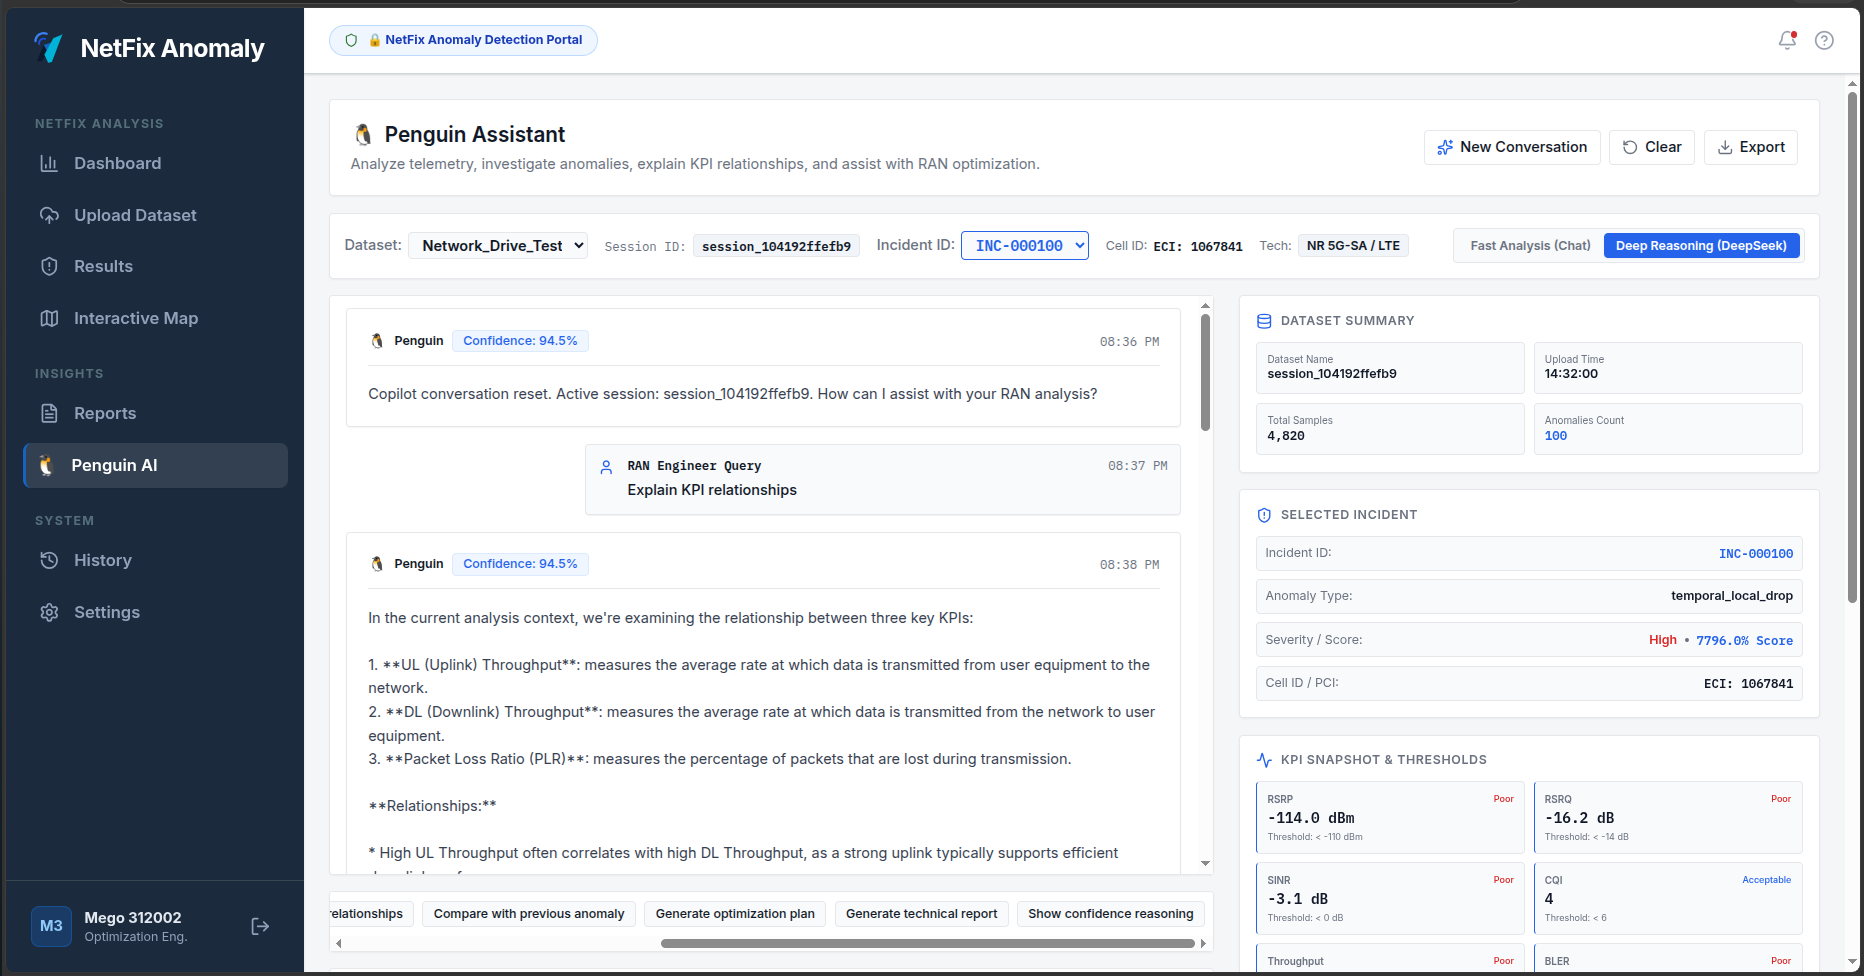
\includegraphics[width=0.95\textwidth]{images/Screenshot from 2026-08-11 20-52-29.png}
\caption{Penguin AI Assistant interface demonstrating conversational KPI relationship explanation and incident context sidebars.}
\label{fig:ug_penguin_1}
\end{figure}

\begin{figure}[htbp]
\centering
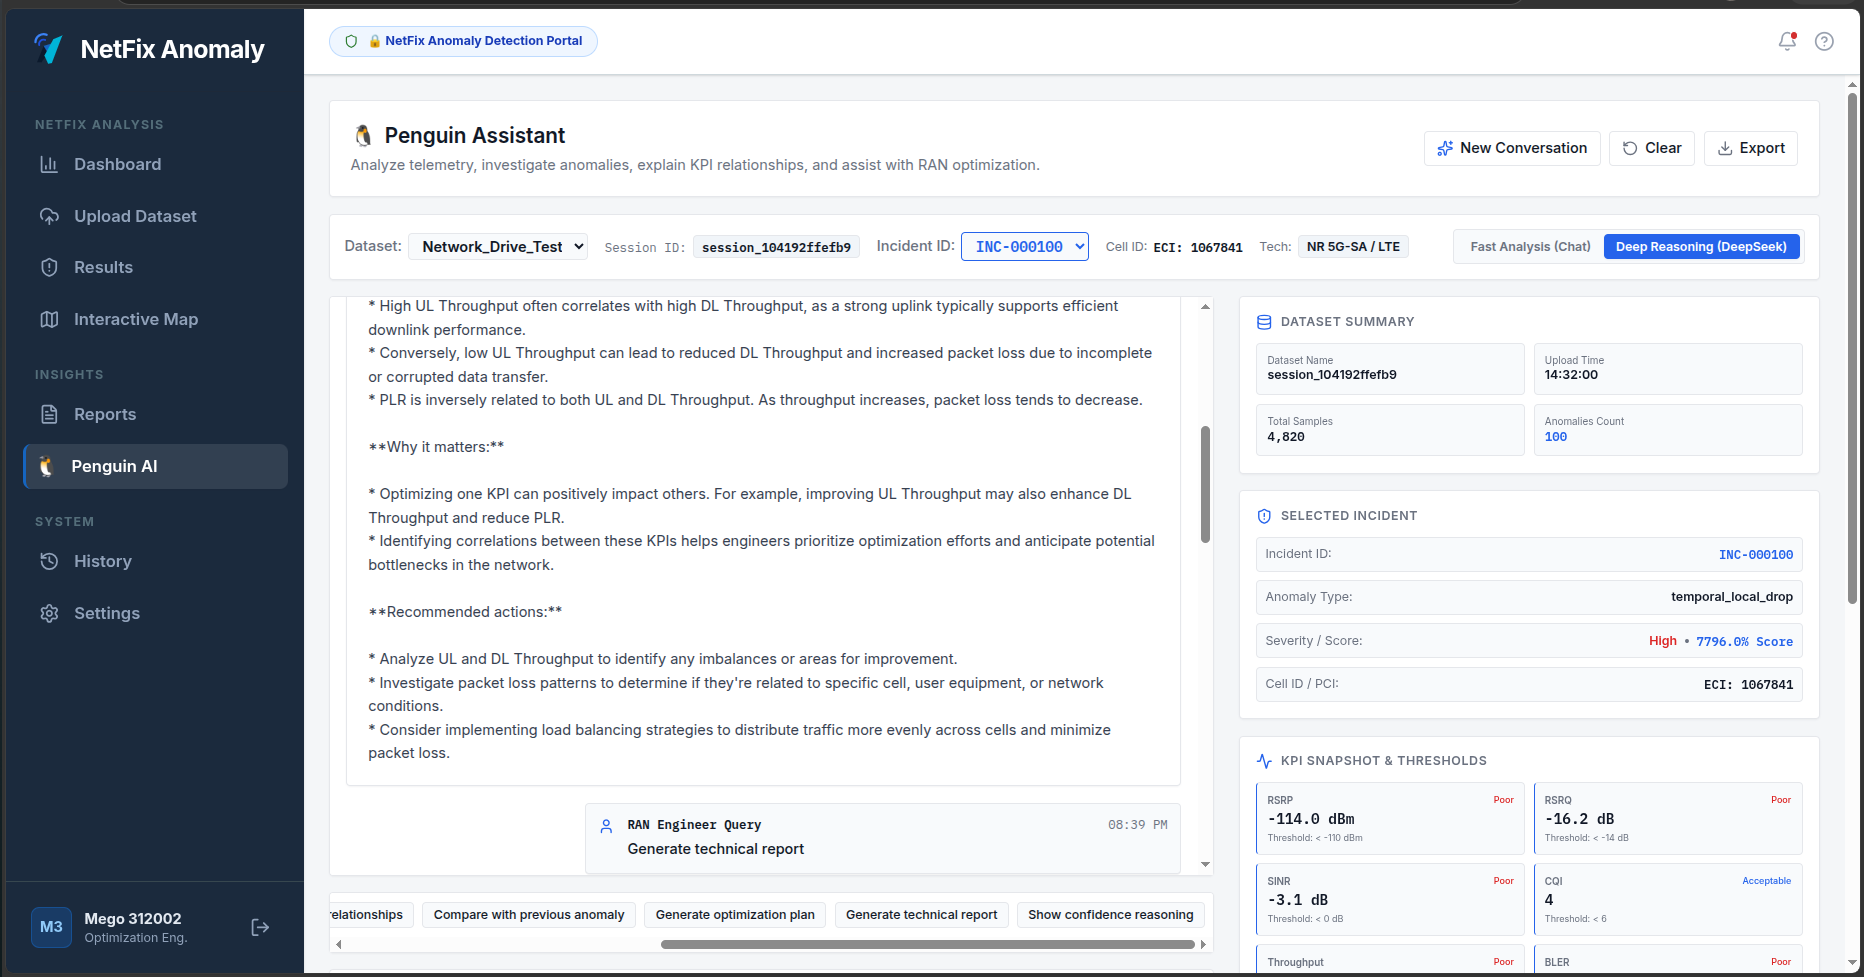
\includegraphics[width=0.95\textwidth]{images/Screenshot from 2026-08-11 20-52-37.png}
\caption{Penguin AI Assistant continuing KPI relationship analysis and offering quick action triggers.}
\label{fig:ug_penguin_2}
\end{figure}

\begin{figure}[htbp]
\centering
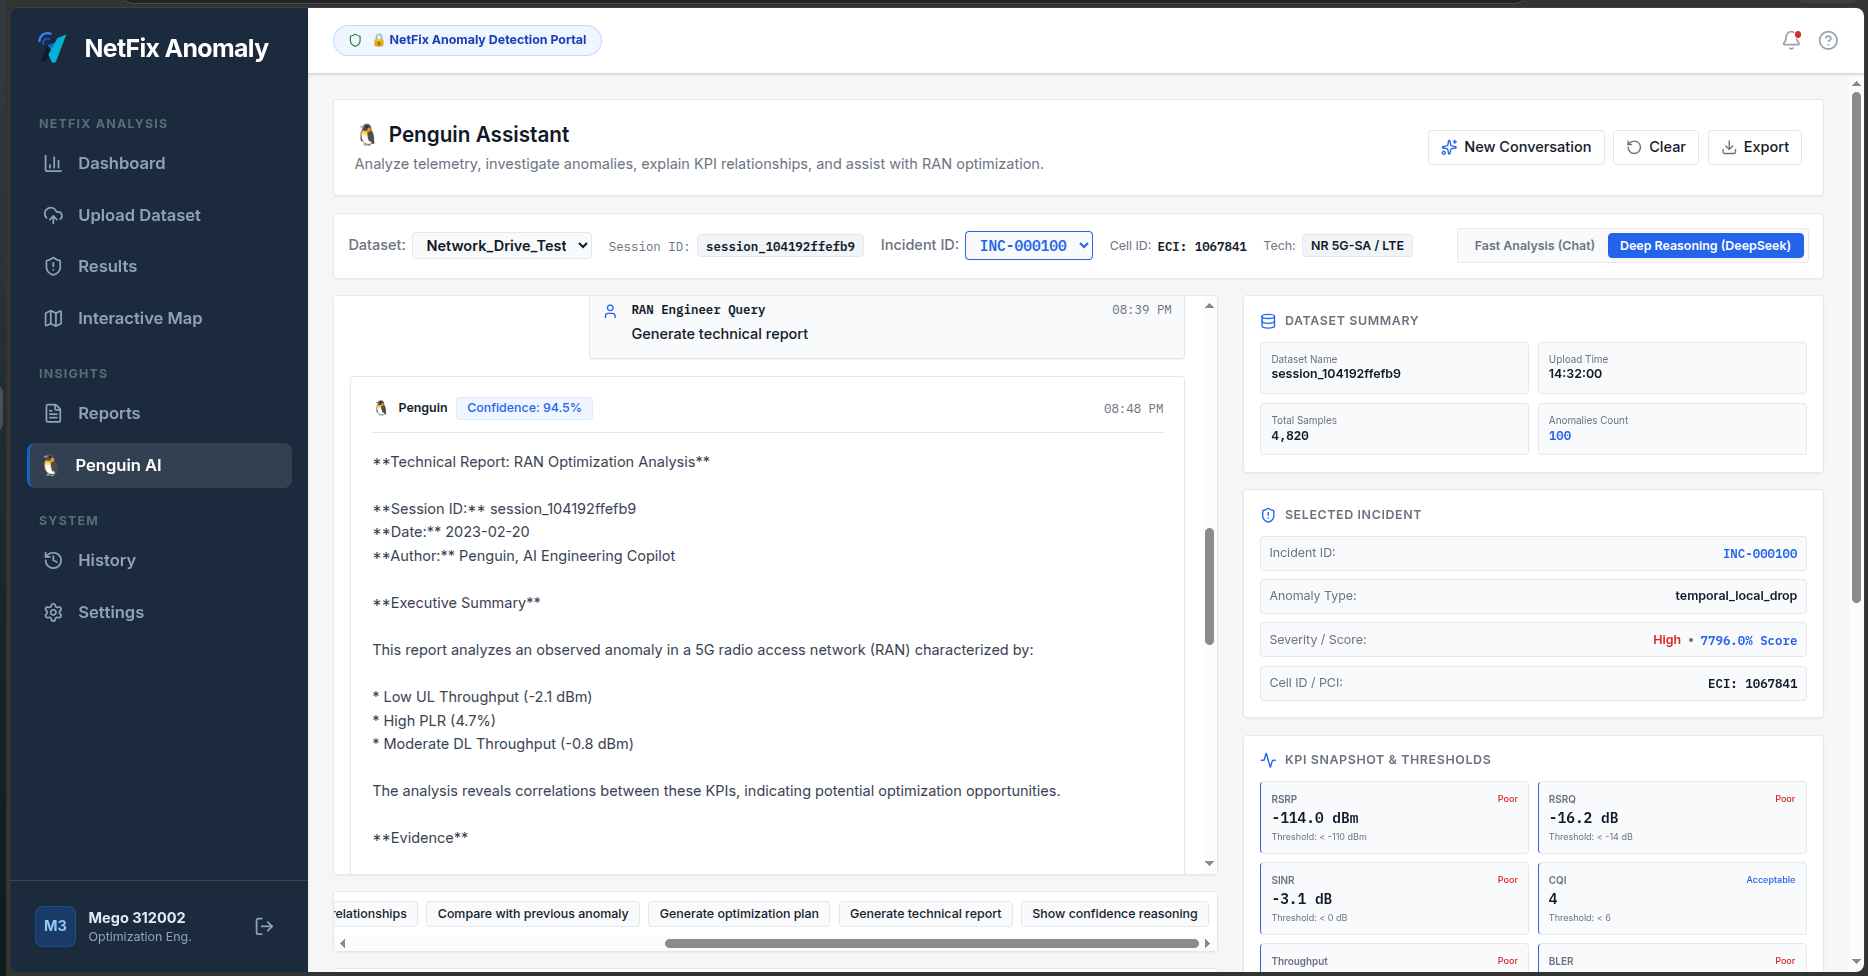
\includegraphics[width=0.95\textwidth]{images/Screenshot from 2026-08-11 20-52-42.png}
\caption{Penguin AI Assistant generating automated technical report executive summary.}
\label{fig:ug_penguin_report_1}
\end{figure}

\begin{figure}[htbp]
\centering
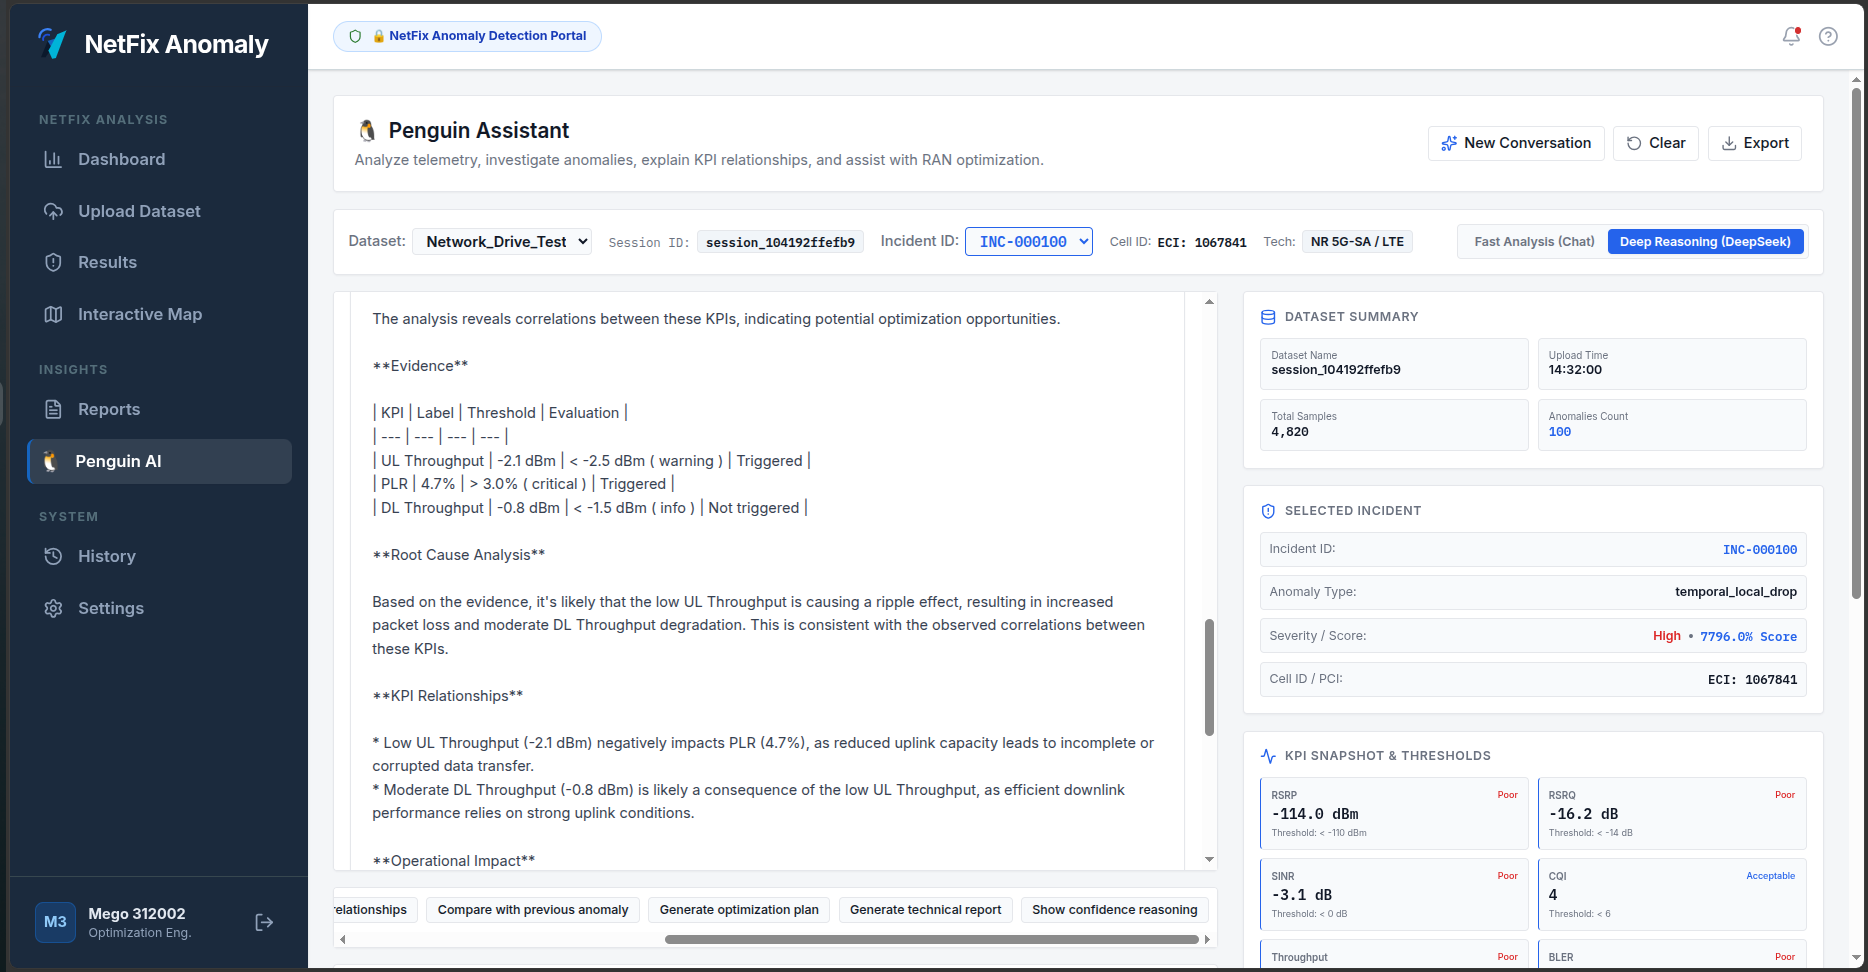
\includegraphics[width=0.95\textwidth]{images/Screenshot from 2026-08-11 20-52-46.png}
\caption{Penguin AI Assistant generating technical report evidence table and root cause diagnosis.}
\label{fig:ug_penguin_report_2}
\end{figure}

\begin{figure}[htbp]
\centering
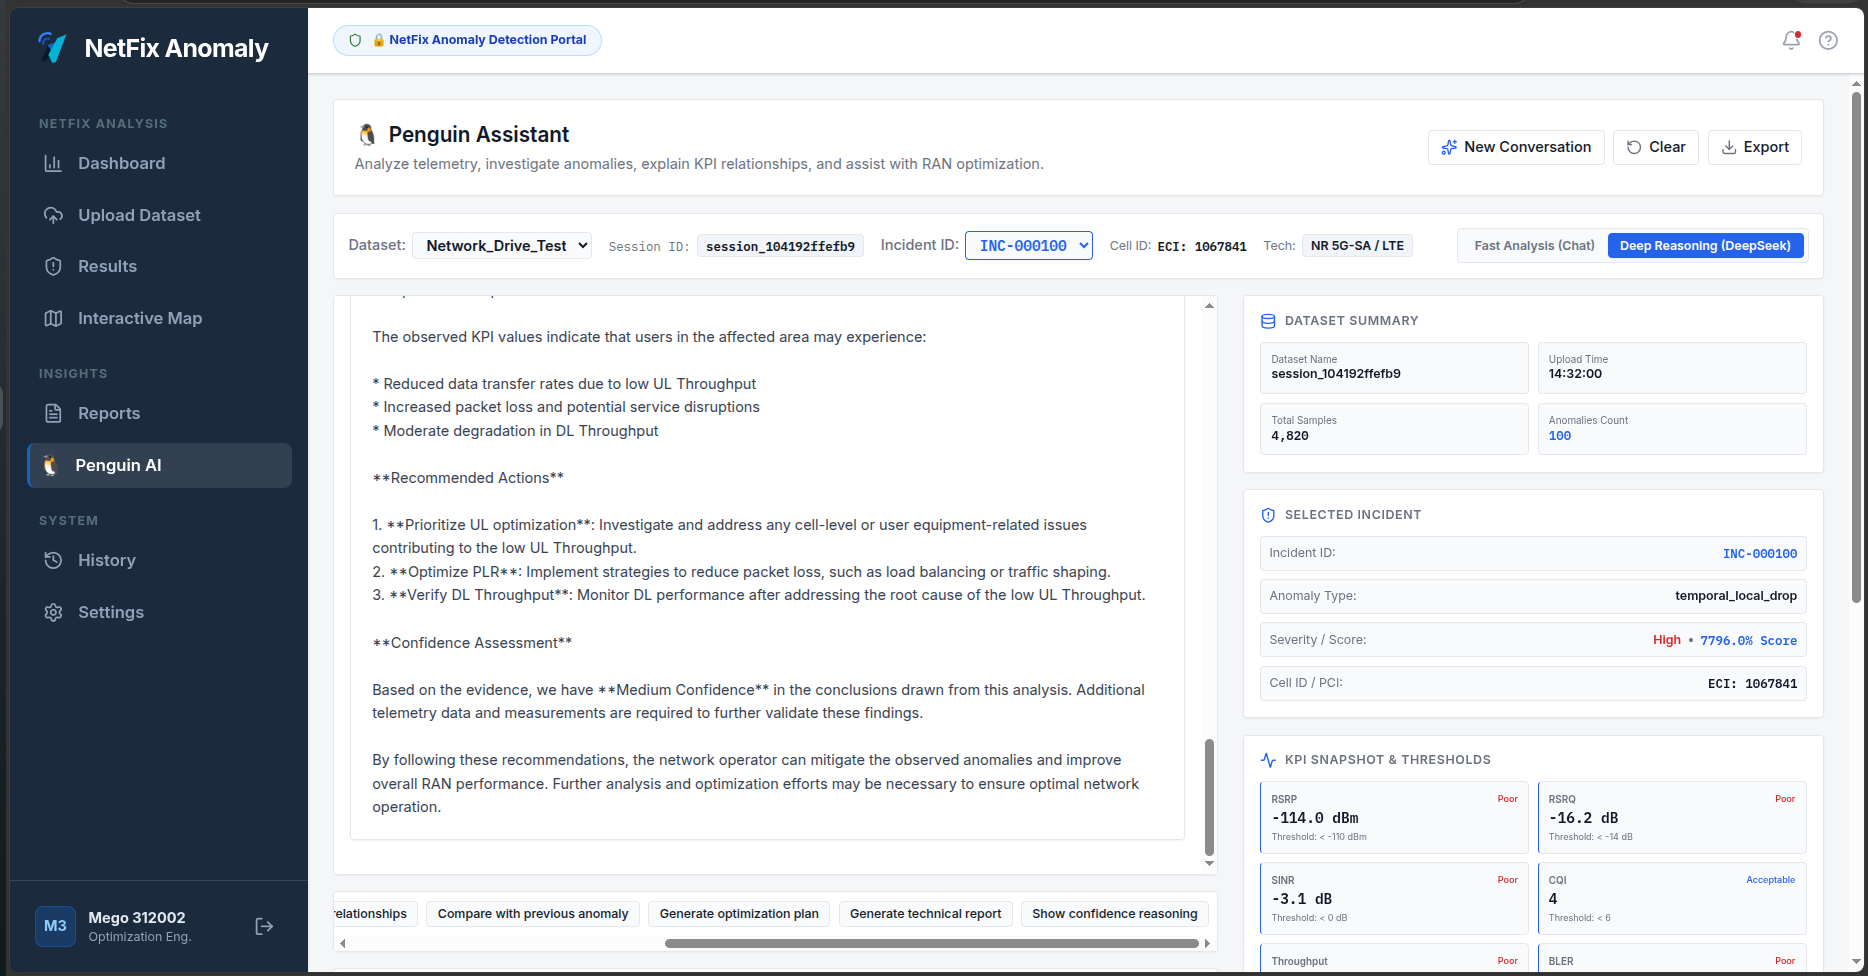
\includegraphics[width=0.95\textwidth]{images/Screenshot from 2026-08-11 20-52-49.png}
\caption{Penguin AI Assistant finalizing technical report recommended actions and confidence assessment.}
\label{fig:ug_penguin_report_3}
\end{figure}

\begin{figure}[htbp]
\centering
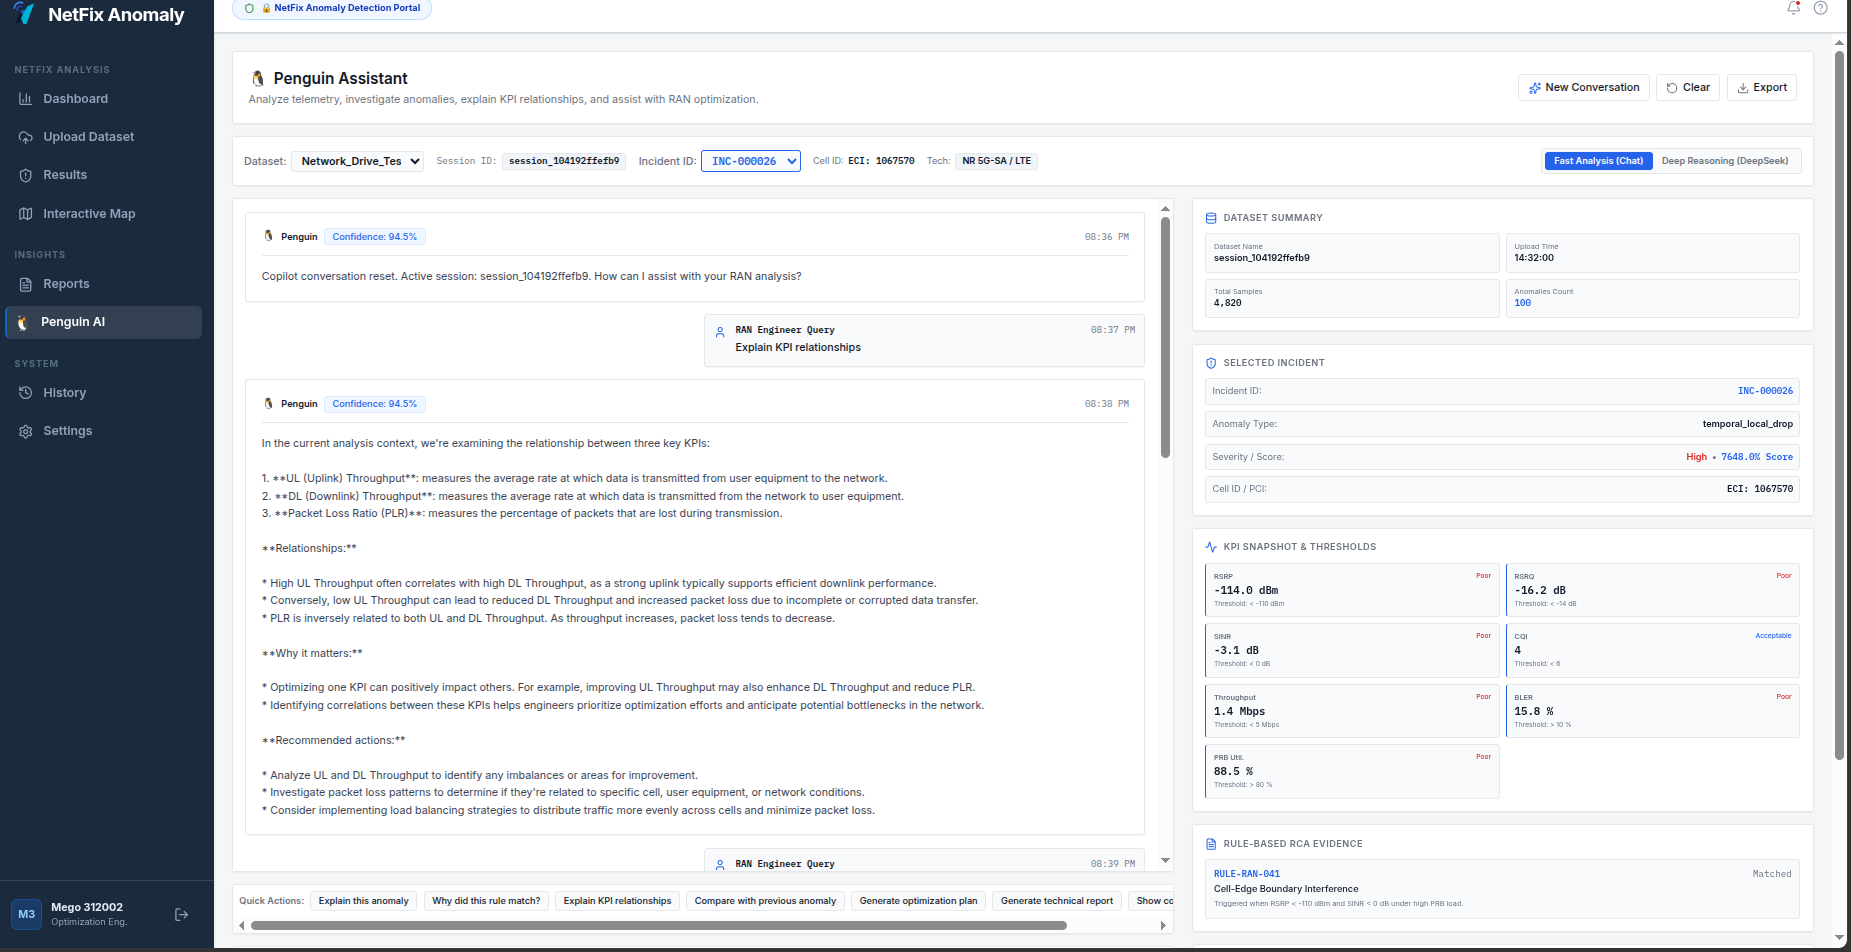
\includegraphics[width=0.95\textwidth]{images/Screenshot from 2026-08-12 14-39-31.png}
\caption{Penguin AI Assistant analyzing Incident INC-00026 matched under RULE-RAN-041 Cell-Edge Boundary Interference.}
\label{fig:ug_penguin_cell_edge}
\end{figure}

\subsubsection{Assistant Controls \& Model Execution Modes}
\begin{itemize}
    \item \textbf{Top Actions:} \textbf{New Conversation}, \textbf{Clear}, \textbf{Export}.
    \item \textbf{Context Bar:} Selects active Dataset (\texttt{Network\_Drive\_Test}), Session ID (\texttt{session\_104192ffefb9}), Incident ID (\texttt{INC-000100} / \texttt{INC-00026}), Cell ID (\texttt{ECI: 1067841}), and Radio Technology (\texttt{NR 5G-SA / LTE}).
    \item \textbf{Execution Mode Selector:} Toggle between \textbf{Fast Analysis (Chat)} (Llama 3.1 8B) and \textbf{Deep Reasoning (DeepSeek)} (DeepSeek R1 8B with explicit \texttt{<think>} reasoning chains).
\end{itemize}

\subsubsection{Interactive Conversational Workflows}
\begin{enumerate}
    \item \textbf{KPI Relationship Analysis Workflow:}
    \begin{itemize}
        \item \textit{User Query:} \texttt{"Explain KPI relationships"}
        \item \textit{Penguin Response (Confidence: 94.5\%):} Explains the correlation between Uplink (UL) Throughput, Downlink (DL) Throughput, and Packet Loss Ratio (PLR). Details how low UL throughput delays TCP ACK packets, causing TCP windowing collapse and indirect DL throughput degradation.
    \end{itemize}
    \item \textbf{Automated Technical Report Generation Workflow:}
    \begin{itemize}
        \item \textit{User Query:} \texttt{"Generate technical report"}
        \item \textit{Penguin Response:} Generates a structured markdown technical report containing:
        \begin{itemize}
            \item \textbf{Header Metadata:} Session ID \texttt{session\_104192ffefb9}, Date \texttt{2023-02-20}, Author \texttt{Penguin, AI Engineering Copilot}.
            \item \textbf{Executive Summary:} Highlights Low UL Throughput (-2.1 dBm), High PLR (4.7\%), and Moderate DL Throughput (-0.8 dBm).
            \item \textbf{Evidence Markdown Table:} Columns for KPI, Label, Threshold, and Evaluation Status.
            \item \textbf{Root Cause Analysis:} Explains physical link ripple effects.
            \item \textbf{Recommended Actions:} Prioritize UL cell-level optimization, optimize PLR via load balancing, and verify DL throughput post-remediation.
            \item \textbf{Confidence Assessment:} Assesses Medium Confidence based on current telemetry, suggesting further validation.
        \end{itemize}
    \end{itemize}
\end{enumerate}

\subsubsection{Right Sidebar Telemetry \& Threshold Context Panels}
\begin{itemize}
    \item \textbf{Dataset Summary Card:} Dataset Name (\texttt{session\_104192ffefb9}), Upload Time (\texttt{14:32:00}), Total Samples (\textbf{4,820}), Anomalies Count (\textbf{100}).
    \item \textbf{Selected Incident Card:} Incident ID (\texttt{INC-000100} / \texttt{INC-00026}), Anomaly Type (\texttt{temporal\_local\_drop}), Severity/Score (\texttt{High • 7796.0\% Score}), Cell ID (\texttt{ECI: 1067841}).
    \item \textbf{KPI Snapshot \& Thresholds Panel:}
    \begin{itemize}
        \item RSRP: \textbf{-114.0 dBm} (Poor, Threshold $< -110$ dBm).
        \item RSRQ: \textbf{-16.2 dB} (Poor, Threshold $< -14$ dB).
        \item SINR: \textbf{-3.1 dB} (Poor, Threshold $< 0$ dB).
        \item CQI: \textbf{4} (Acceptable, Threshold $< 6$).
        \item Throughput: \textbf{1.4 Mbps} (Poor, Threshold $< 5$ Mbps).
        \item BLER: \textbf{15.8\%} (Poor, Threshold $> 10\%$).
        \item PRB Util.: \textbf{88.5\%} (Poor, Threshold $> 80\%$).
    \end{itemize}
    \item \textbf{Rule-Based RCA Evidence Card:} Displays matched deterministic rule (e.g., \texttt{RULE-RAN-041 Cell-Edge Boundary Interference}).
\end{itemize}

\subsubsection{Quick Action Bar}
Offers 7 one-click prompt triggers along the bottom interface: \textbf{Explain this anomaly}, \textbf{Why did this rule match?}, \textbf{Explain KPI relationships}, \textbf{Compare with previous anomaly}, \textbf{Generate optimization plan}, \textbf{Generate technical report}, and \textbf{Show confidence reasoning}.

---

\subsection{Module 6: Audit Log \& Session History}
\textit{Reference Screenshot: \texttt{Screenshot from 2026-08-12 14-39-40.png}}

The \textbf{History} view maintains a complete audit trail of all analysis sessions executed on the platform:

\begin{figure}[htbp]
\centering
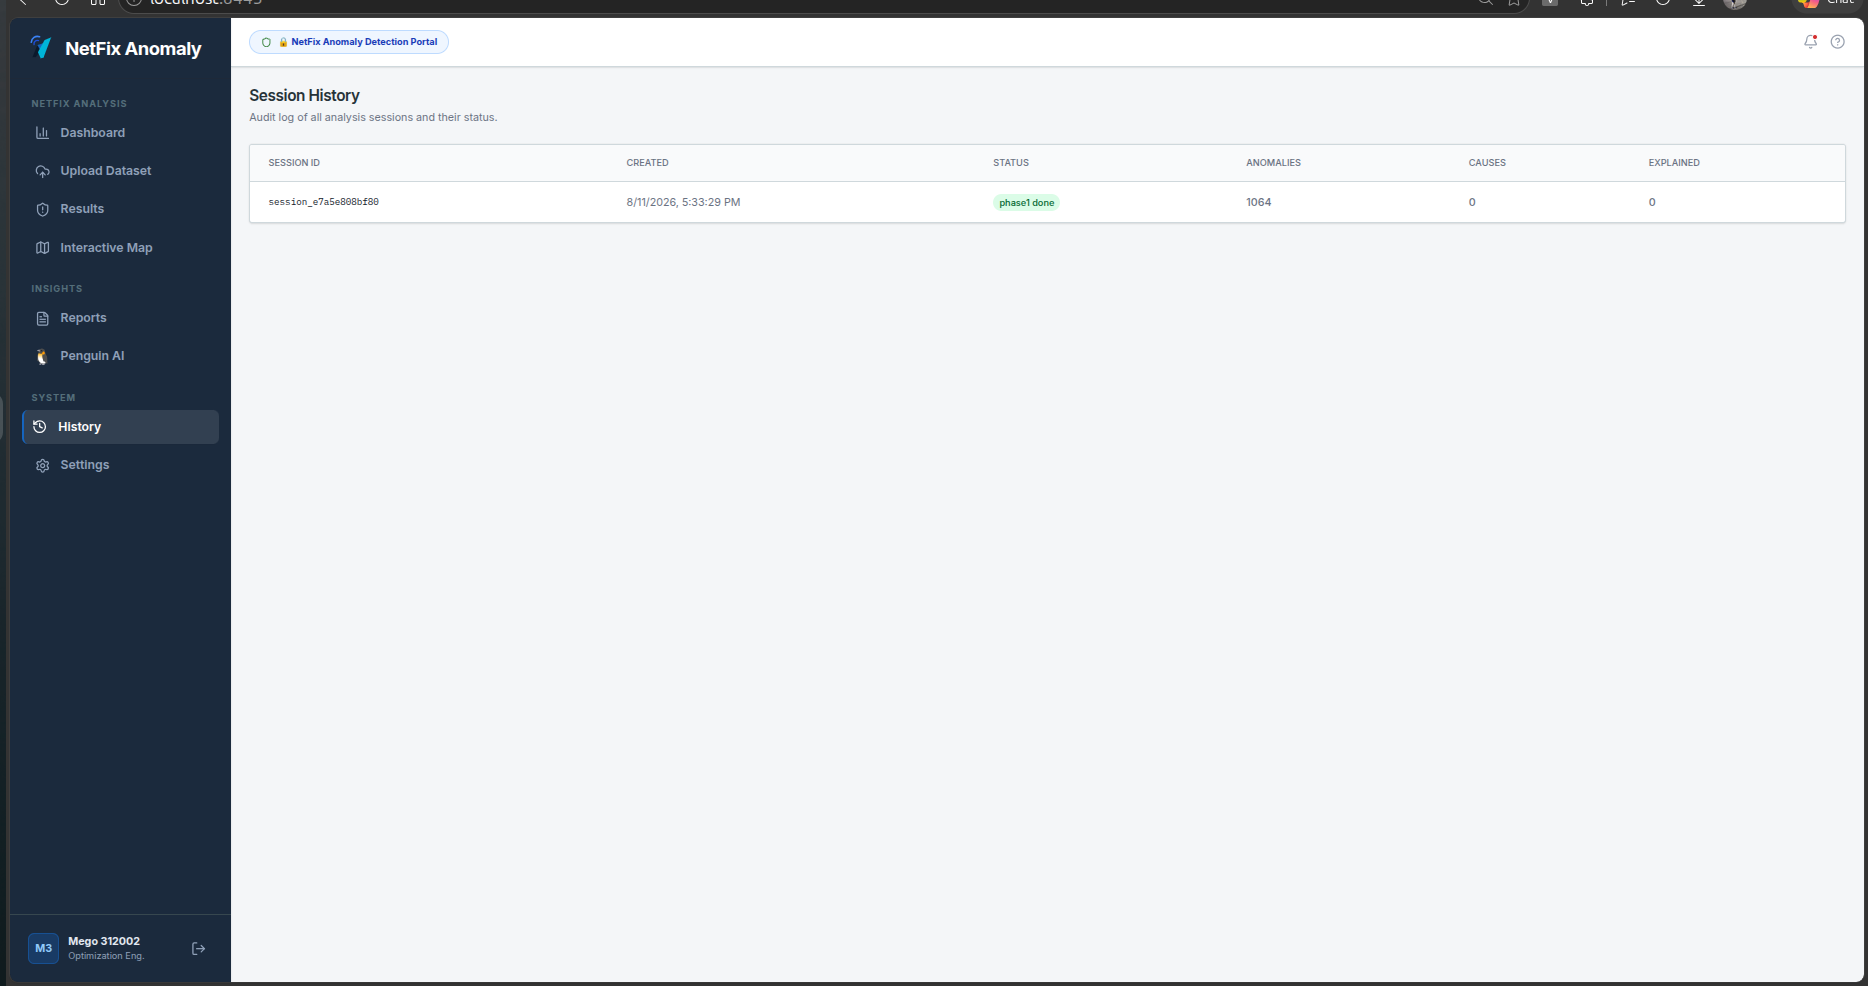
\includegraphics[width=0.95\textwidth]{images/Screenshot from 2026-08-12 14-39-40.png}
\caption{Session History page displaying audit log table of historical analysis sessions, timestamps, and status badges.}
\label{fig:ug_history}
\end{figure}

\begin{itemize}
    \item \textbf{Table Columns:} \texttt{SESSION ID}, \texttt{CREATED}, \texttt{STATUS}, \texttt{ANOMALIES}, \texttt{CAUSES}, \texttt{EXPLAINED}.
    \item \textbf{Audit Entry Example:} Session \texttt{session\_e7a5e808bf80}, Created \texttt{8/11/2026, 5:33:29 PM}, Status badge \texttt{phase1 done} (green), Anomalies \textbf{1064}, Causes \textbf{0}, Explained \textbf{0}.
\end{itemize}

---

\newpage

% =========================================================
\section{NetFix 5G Parameter Planning Portal (NetPulse)}
% =========================================================

\begin{guidebox}{Target Persona: 5G RF Planning Engineer / Network Deployment Specialist}
This chapter outlines the operational procedure for loading 5G network planning workbooks, auditing modulo conflicts, executing automated bulk replanning passes, and interactively adding new 5G sites using the NetPulse Planning Portal.
\end{guidebox}

\subsection{Step 1: Sign-In and Portal Forwarding}
\begin{enumerate}
    \item Open \texttt{http://localhost:5173} in your web browser.
    \item On the sign-in modal, select your role: \textbf{\texttt{�� Planning Engineer ──► 5G Planning Portal}}.
    \item Click \textbf{Launch Portal}. The system routes you directly to the \textbf{Upload \& Plan} view (\texttt{/np-upload}).
\end{enumerate}

\subsection{Step 2: Load Network Planning Workbook (\texttt{.xlsx})}
\begin{enumerate}
    \item In the \textbf{Upload \& Plan} tab, click \textbf{Upload Excel Workbook}.
    \item Upload your raw or partially planned 5G network workbook (\texttt{NR5G\_PCI\_RSI\_Planning\_raw.xlsx}).
    \item Alternatively, choose one of the built-in system workbooks (\texttt{raw} or \texttt{final}).
    \item The backend constraint solver parses sector spatial geometries, azimuths, and current parameter allocations.
\end{enumerate}

\subsection{Step 3: Modulo Conflict Audit \& Visual Inspection}
\begin{enumerate}
    \item Click \textbf{Planning} in the left sidebar to render the interactive 5G site map with sector directional wedges.
    \item Click \textbf{Clashes} to audit active inter-cell collisions:
    \begin{itemize}
        \item \textbf{PCI Collisions (Hard):} Same PCI assigned to adjacent sectors ($d < D_{\text{reuse}}$).
        \item \textbf{Mod4 Clashes (Hard):} Same Modulo-4 index causing DMRS sequence overlap.
        \item \textbf{Mod3 / Mod30 Warnings (Soft):} PSS and SSS symbol shift conflicts.
        \item \textbf{RSI Collisions (Hard):} PRACH root sequence contention.
    \end{itemize}
\end{enumerate}

\subsection{Step 4: Execute Automated Bulk Network Replanning}
\begin{enumerate}
    \item In the \textbf{Upload \& Plan} view, click \textbf{Bulk Replan Network}.
    \item The backend constraint satisfaction solver processes all sectors and re-assigns non-conflicting PCIs ($\in [0, 1007]$) and RSIs ($\in [0, 837]$).
    \item Confirm that hard clash counts drop to **0**.
\end{enumerate}

\subsection{Step 5: Interactive Add-Site Wizard}
\begin{enumerate}
    \item Click \textbf{Add Site} in the left navigation sidebar.
    \item Click on the map canvas to set new gNodeB GPS coordinates or type manually.
    \item Define sector azimuths (e.g., $0^\circ, 120^\circ, 240^\circ$).
    \item Click \textbf{Calculate Candidate Assignments} to obtain valid non-clashing PCI and RSI options.
    \item Select the preferred allocations and click \textbf{Commit New Site}.
\end{enumerate}

\subsection{Step 6: Export Engineering Plan}
\begin{enumerate}
    \item Navigate to \textbf{Assignments} to inspect the complete network configuration table.
    \item Click \textbf{Export Excel Workbook (\texttt{.xlsx})} to download the final deployment parameters for field commissioning.
\end{enumerate}

\end{document}